
Navigation data in satellite communication refers to the crucial information transmitted between satellites and ground-based receivers to facilitate accurate positioning and navigation. It includes data related to satellite orbits, precise timing, and other parameters necessary for determining the satellite's position relative to the Earth's surface.
\section{Frame structure}
The NavIC L1 Master Frame is of $1800$ symbols long made of $3$ subframes. Subframe $1$ consists of $52$ symbols, Subframe $2$ is composed of 1$200$ symbols, and Subframe$3$ is comprised of $548$ symbols,The master frame structure is shown in figure \ref{fig:master_frame}


\begin{figure}[ht]
\centering
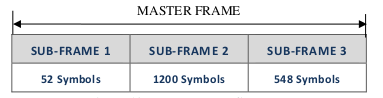
\includegraphics[width=0.8\columnwidth]{figs/master_frame}
\centering
\captionsetup{justification=centering}
\caption{Master Frame Structure}
\label{fig:master_frame}
\end{figure}


The Time of Interval (TOI)is transmitted in Subframe 1 is shown in figure \ref{fig:subframe1}. Subframe $2$ as shown in figure \ref{fig:subframe2}, transmitting the primary navigation parameters, and Subframe $3$ is shown in figure \ref{fig:subframe3}responsible for transmitting secondary navigation parameters.The secondary navigation parameters are transmitted in message format.It identifies the message types that the NavIC satellites will transmit. Provision exists to define new messages for future requirements in NavIC. Each message is identified by a unique message identifier.
 


\begin{figure}[ht]
\centering
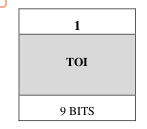
\includegraphics[width=0.4\columnwidth]{figs/subframe1.png}
\centering
\captionsetup{justification=centering}
\caption{ Sub-frame 1 Layout}
\label{fig:subframe1}
\end{figure}

\begin{figure}[ht]
\centering
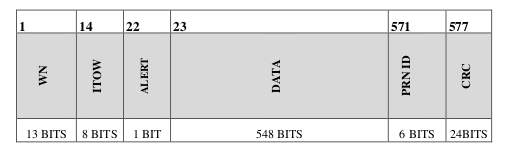
\includegraphics[width=0.8\columnwidth]{figs/subframe2.png}
\centering
\captionsetup{justification=centering}
\caption{Sub-frame 2 Layout}
\label{fig:subframe2}
\end{figure}

\begin{figure}[ht]
\centering
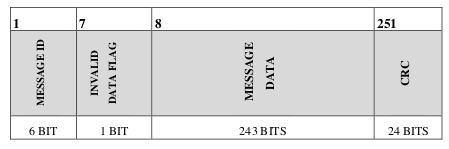
\includegraphics[width=0.8\columnwidth]{figs/subframe3.png}
\centering
\captionsetup{justification=centering}
\caption{Sub-frame 3 Layout}
\label{fig:subframe3}
\end{figure}
\subsection{L1 SPS DATA STRUCTURE}
The NavIC Signal-In-Space transmits navigation message data through the SPS service, in the L1 band. The sub-frame structure is shown in Figure \ref{fig: SPS_Structure}
\begin{figure}[ht]
\centering
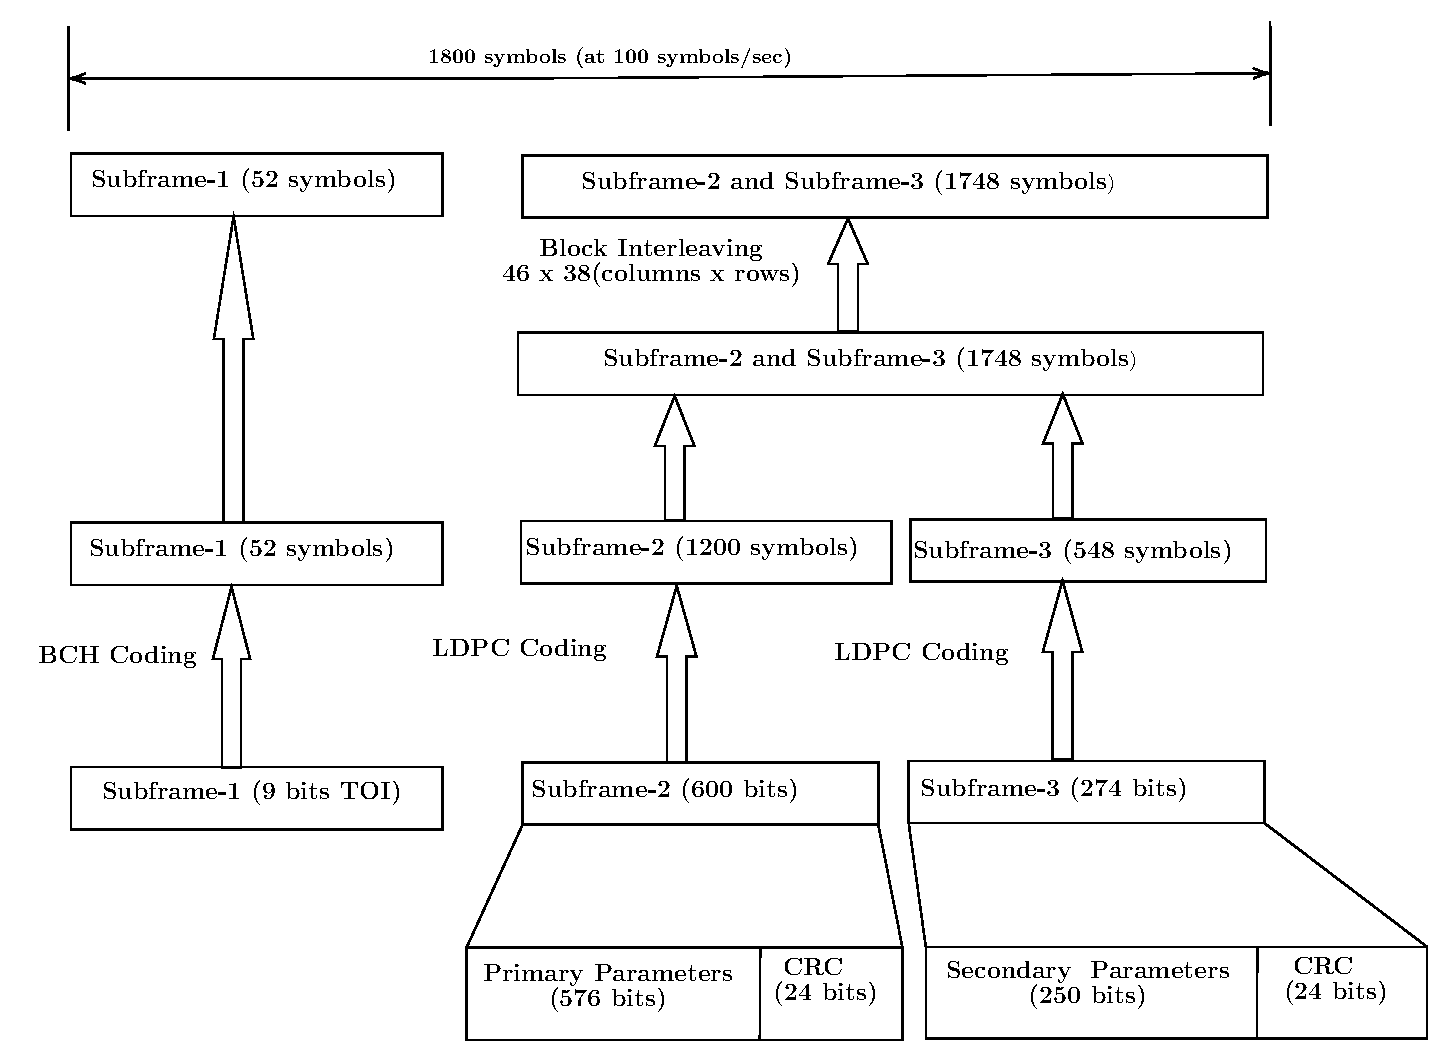
\includegraphics[width=0.8\columnwidth]{figs/spsframe}
\centering
\captionsetup{justification=centering}
\caption{NavIC L1 SPS Subframe Structure}
\label{fig: SPS_Structure}
\end{figure}

\noindent The 600 bits of subframe $2$ and $274$ bits of subframe $3$ are Low Density Parity Check (LDPC) Forward Error Correction (FEC) encoded and interleaved as shown in Figure \ref{fig: SPS_Structure}. Subframe $2$ and subframe $3$ are separately encoded using rate $\frac{1}{2}$ Quasi Cyclic LDPC codes.
Subframe $1$ consists of $9$ bits that are Bose, Chaudhuri, and Hocquenghem (BCH) encoded.
Subframe $2$ has a total of $600$ bits, comprising $576$ bits for primary navigation parameters and $24$ bits for CRC.
Subframe $3$ contains a total of $274$ bits, with $250$ bits for secondary navigation parameters and $24$ bits for CRC.
sAs a result of rate $\frac{1}{2}$ Quasi Cyclic LDPC encoding, there are $1200$ symbols (coded bits) for subframe $2$ and $548$ symbols for subframe $3$, as described in Figure \ref{fig: SPS_Structure}.

\section{Cyclic Redundancy Check(CRC)}
The parity coding of data signal follows $24$Q polynomial for each subframe. $24$ bits of CRC parity will provide protection against burst as well as random errors with undetected error probability of $2^{-24}$ for all channel bit error probabilities $0.5$.
\begin{equation}
    g(X) = \sum_{i = 0}^{24}g_{i}X^i\;\; 
\end{equation}

    $g_{i}=1$; for $i = 0,1,3,4,5,6,7,10,11,14,17,18,23,24$ \\
          = 0 otherwise

\let\cleardoublepage\clearpage
